\section{Problems}
\label{section:behavModelsProblems}

\begin{enumerate}
\def\labelenumi{\arabic{enumi}.}
\item
  Why is it important for a model to separate the design of a system
  from its realization?

  \begin{onlysolution}
    \textbf{[R]}
    \itshape
    Separating the design from its realization allows the designer to see the 
    forest instead of the trees. That is, working with models which abstract away 
    the details of the implementation allows a designer see the entire system as a 
    whole with being distracted by the individual parts. Furthermore, it allows the 
    design to change the way the components are implemented. Thus, if a better 
    technology emerges during the course of the design, the implementation of the 
    component can be changed without affecting the overall design.
  \end{onlysolution}
\item
  Classify each of the following as either a model, not a model, or
  sometimes a model. Justify your answer based on the definition and
  properties of a model.

  \begin{onlysolution}
    \textbf{[R]}
    \itshape
  \end{onlysolution}

\begin{itemize}
  \def\labelenumi{\alph{enumi})}
  \item A diagram of a subway system,

    \begin{onlysolution}
      \textbf{[R]}
      \itshape
      A diagram of a subway system is a model because it is an abstract 
      simplification of the physical subsystem. It’s abstract because it’s 
      not the actual subway system; it’s just a printed piece of paper. It’s 
      a simplification because it removes lots of unnecessary details in 
      order to facilitate communication. For example, most subway diagrams are 
      not to scale, nor do they show the actual orientation of the railways.
    \end{onlysolution}

  \item a computer program, 

    \begin{onlysolution}
      \textbf{[R]}
      \itshape
      A program is sometimes a model. A program modeling a physical process like 
      a gravitational attraction of a three body system is an abstract simplification 
      of a three interstellar bodies floating around in space. On the other hand, 
      a program which sorts number is not necessarily a model of anything; it’s just 
      used to sort number.
    \end{onlysolution}

  \item a football play, 

    \begin{onlysolution}
      \textbf{[R]}
      \itshape
      A football play is a model. It’s an abstraction simplification of the physical 
      system. It’s abstract because its written on paper, the X’s and O’s represent 
      actual football players.
    \end{onlysolution}

  \item drivers license,

    \begin{onlysolution}
      \textbf{[R]}
      \itshape
      A driver’s license is not a model. The information contained on the license describes 
      a person and so to some extent is an abstraction of a person. However, its not the 
      intent of the driver’s license to be a model of a person, rather its intention is that 
      it contain enough data make a unique association between a person and a privilege.
    \end{onlysolution}

  \item a floor plan of the local shopping mall (a ``you are here'' diagram)., 

    \begin{onlysolution}
      \textbf{[R]}
      \itshape
      A floor plan is a model because it’s a simplification of the actual shopping 
      complex, its just a print out on paper. It’s an abstraction because many of 
      the real details of the shopping mall are not shown, like the doorways, lights, 
      and the ubiquitous mall water fountain.
    \end{onlysolution}

  \item an equation, 

    \begin{onlysolution}
      \textbf{[R]}
      \itshape
      An equation is sometimes a model. The Newtonian equation representing the position 
      of a falling body in a constant gravitational field is an abstract representation of 
      a real falling body. It’s a simplification because it neglects things like air 
      resistance. However, an equation of a parabola is not necessarily an abstract 
      representation of anything, it’s just a parabola.
    \end{onlysolution}

  \item A scratch n' sniff perfume advertisement in a fashion magazine,

    \begin{onlysolution}
      \textbf{[R]}
      \itshape
      Is a model because it captures the essential characteristic of perfume 
      (its smell) without specifying how the perfume will produced.
    \end{onlysolution}

  \item The 1812 overture,

    \begin{onlysolution}
      \textbf{[R]}
      \itshape
      Tchaikovsky (a Russian) was commissioned to write this piece of music to commemorate 
      Napoleon’s unsuccessful 1812 invasion into Russia. The musical score follows the 
      progression of this conflict at times even calling for live cannon fire. So we could 
      call the 1812 overture a simplified representation of the Napoleonic invasion and 
      hence it is a model.
    \end{onlysolution}

  \item a braille sign reading ``second floor'',

    \begin{onlysolution}
      \textbf{[R]}
      \itshape
      It not a model for two reasons. While Braille forms representations for letters, the 
      symbol string isn’t a simplification because each Braille symbol has a one-to-one 
      correspondence to a letter. The information contained in the message is not an effective 
      simplification of the building’s structure; we can only know that the building has at 
      least two floors.
    \end{onlysolution}

  \item sheet music for the Brandenburg Concerto, 

    \begin{onlysolution}
      \textbf{[R]}
      \itshape
      Sheet music in almost any form is a model because it’s a simplification of an actual 
      musical performance written in a standardized language.
    \end{onlysolution}

  \item the United States Constitution, 

    \begin{onlysolution}
      \textbf{[R]}
      \itshape
      The US constitution is a model of a government. It’s a simplification because it 
      does not try to capture all details of the eventual government, but rather establishes 
      a framework for the structures and organization of a government.
    \end{onlysolution}

  \item a set of car keys,

    \begin{onlysolution}
      \textbf{[R]}
      \itshape
      Car keys are not a model. They are not representative of anything and are not a simplification.
    \end{onlysolution}

  \item the ASCII encoding of an email message.

    \begin{onlysolution}
      \textbf{[R]}
      \itshape
      Is not a model.
    \end{onlysolution}

\end{itemize}


\item
  Which of the following systems has memory? Justify your answer using
  the concepts of input, output, and state.
  \begin{itemize}
    \def\labelenumi{\alph{enumi})}
    \item  an ink pen,

      \begin{onlysolution}
        \textbf{[R]}
        \itshape
        An ink pen has memory. Let the input be the process of writing with the pen. 
        Let the output be visible text. The same input can cause different output 
        depending on the level of ink in the pen, empty or not empty. Sometimes a state 
        variables (like ink level) are referred to as hidden variables, because if their 
        value were know then the system would not appear to have state. For example if 
        you had a see-through pen then it would be reasonable to assume that the ink level 
        could be observed prior to writing and consequently could be considered to be an 
        input to the system.
      \end{onlysolution}

    \item a resistor,

      \begin{onlysolution}
        \textbf{[R]}
        \itshape
        A resistor does not have memory. Let the input to the resistor be current and let 
        the output be voltage. A given current always produces the same voltage drop across 
        the resistor, regardless of what has happen in the past.
      \end{onlysolution}
    
    \item a capacitor,

      \begin{onlysolution}
        \textbf{[R]}
        \itshape
        A capacitor has memory. Let the input be voltage and the output current. The 
        relationship between these two is characterized by the equation, I=Cdv/dt. The graphs 
        below represent a time varying voltageapplied across a capacitor. Note that the voltage 
        measured at time t0 and t1 are the same, vref. However, the current through the cap will 
        be different at times t0 and t1 because the slope of the voltage vs. time graph is different.
        ** Add figure ** 
      \end{onlysolution}

    \item a motorized garage door,

      \begin{onlysolution}
        \textbf{[R]}
        \itshape
        A motorized garage door has memory. Let the input be the button press to activate door movement, 
        the output be the movement of the door, and the state variable be the position of the door. 
        When the button is pressed the direction of the door’s movement (opening or closing) depends 
        on weather the door was open or closed.
      \end{onlysolution}

    \item an analog wrist watch, 

      \begin{onlysolution}
        \textbf{[R]}
        \itshape
        An analog wrist watch has memory. The input is time and the output is the indicated time. The output 
        is determine by the passage of time and the value of the previous time.
      \end{onlysolution}

    \item the air pressure in an air compressor, 

      \begin{onlysolution}
        \textbf{[R]}
        \itshape
        The air pressure itself does not have memory, but the air compressor does have memory. Compressors have 
        a high and low pressure threshold. When the pressure in the compressor tank falls below the low threshold, 
        the air pump automatically turns on, increasing the pressure in the tank. When the pressure in the tank 
        exceeds the high pressure threshold the compressor turns off. When the pressure is between the two thresholds 
        the compressor keeps doing what it had been doing moments before.
      \end{onlysolution}

    \item  the thermostat which controls the furnace in a house,
    
      \begin{onlysolution}
        \textbf{[R]}
        \itshape
        The thermostat to control your house furnace has memory. When you set the temperature of a thermostat you are 
        really setting two temperatures, a low threshold and a high threshold. When the temperature falls below the low 
        threshold the furnace turns on heating the house. When the temperature rises below the high threshold the 
        furnace turns off cooling the house. When the temperature is between the two thresholds the furnace keeps doing 
        what it had be doing moments before. The input is the temperature, the output the state of the furnace, and the 
        state variable the previous state of the furnace.
      \end{onlysolution}

    \item a light switch, 

      \begin{onlysolution}
        \textbf{[R]}
        \itshape
        A common 1-way light switch doesn’t have state – the position of the switch determines the state of the light. 
        A 2-way switch does have state. 2-way switches are used in homes to control a stairwell light from either the 
        top or bottom of the stairs. Let the input be the position of the light switch at the bottom of the stairs, 
        the output be the state of the light bulb, and the state variable be the position of the light switch at the 
        top of the stairs.
      \end{onlysolution}

    \item a political system,

      \begin{onlysolution}
        \textbf{[R]}
        \itshape
        Political systems should have memory. For example, a bill to fund the local puppy shelter is not passed. Irate 
        voters take their let their representatives know about their displeasure. The same bill coming up a year later 
        is more likely to pass.
      \end{onlysolution}

    \item the temperature of a large lake, 

      \begin{onlysolution}
        \textbf{[R]}
        \itshape
        The temperature of a large lake has memory. Let the input be the amount of light falling on a lake and the output 
        be the temperature of the lake. In the northern United States lakes will reach their peak temperature in late August 
        or early September whereas sunlight intensity peaks on the summer solstice (around June 21). Even the surface air 
        temperatures peak in late July or early August, about a full month ahead of the peak lake temperatures.
      \end{onlysolution}

    \item a book, 

      \begin{onlysolution}
        \textbf{[R]}
        \itshape
        Books don't have memory.
      \end{onlysolution}

    \item a computer's hard drive.

      \begin{onlysolution}
        \textbf{[R]}
        \itshape
        A computer hard drive has memory because a byte read from a location depends on what has been written to the drive 
        in the past.
      \end{onlysolution}

  \end{itemize}

  \item
    A can of soda has memory. Your objective is to figure out what
    characteristic of the can is the state variable and what input
    causes it to change. Based upon this, draw a state diagram for a can
    of soda. Label the transition arcs with the input responsible for
    the transition. Hint: no special equipment is needed to elicit the
    change of state.

    \begin{onlysolution}
      \textbf{[R]}
      \itshape
      We will use the “internal pressure” of the can as the state variable. When you shake a can of soda vigorously you 
      “pressurize” it. In order to decrease the pressure, all you need to do is wait. The can of soda has state because 
      it remembers previous input; did you recently shake the can? Opening the can will reveal which of the two states 
      it is in.
      ** Add figure **
    \end{onlysolution}

  \item
    Consider the state diagram for the vending machine shown in 
    Table~\ref{table:stateVendingMachine}.
    Now assume that the system accepts nickels, dimes, and
    quarters. Also assume that it is capable of returning change to the
    user after a purchase. Create a state diagram that represents this
    new system. Make sure to define the output signals and their value
    for each state.

    \begin{onlysolution}
      \textbf{[R]}
      \itshape
      ** Add figures / solution ** 
    \end{onlysolution}

  \item
    Use a state diagram to describe the high level operation of the
    ChipMunk Recorder (CMR). The CMR records sounds and then plays them
    back at a variety of speeds, making a recorded voice sound like a
    high pitched chipmunk. The CMR receives user input from a keyboard
    and an audio source. The behavior of the system is described as
    follows:
\begin{itemize}
\item
  When powered up, the CMR enters a wait state.
\item
  If \textquotesingle R\textquotesingle{} is pressed the recorder begins
  recording.
\item
  Any key-press will put the CMR back into the wait state.
\item
  If \textquotesingle S\textquotesingle{} is pressed, the CMR is ready
  to change the playback speed. A subsequent numerical input between 1
  and 5 will cause the playback speed to be changed to that value.
\item
  Pressing the \textquotesingle R\textquotesingle{} key when in the
  adjust playback speed mode will cause the CMR to go to the wait state.
\item
  Pressing a \textquotesingle P\textquotesingle{} key will cause the CMR
  to playback the recorded sounds. When done playing the entire
  recording, the CMR will loop back and start playing at the beginning.
\item
  Any key-press while in the playback mode will cause the CMR to go back
  into the wait state.
\end{itemize}

  Draw a state diagram describing the behavior of the CMR. Create a
  table which lists every state and its associated output.

  \begin{onlysolution}
    \textbf{[R]}
    \itshape
    ** Add figures **
  \end{onlysolution}

  \item
  \label{problem:stateDiagramTapeCartridges}
    Build a state diagram to describe the state of the tape cartridges
    used to backup a company's network drives. When new
    \textbf{unformatted} cartridges are received they are immediately
    labeled with a unique ID. Before a tape is used it is formatted
    turning it into a \textbf{blank} tape. On the first day of the week
    a complete backup is made of the network drives, transforming blank
    tapes into \textbf{active} tapes. The active tapes, made every
    fourth week, are moved off site making them \textbf{archival} tapes.
    Active tapes older than 3 months are assumed to have out of date
    information and are reformatted into blank tapes. Archival tapes
    more than 2 years old are reformatted and put back into circulation.

    \begin{onlysolution}
      \textbf{[R]}
      \itshape
      ** Add figures **
    \end{onlysolution}

  \item
    Build a flowchart to describe the operation of a microcontroller
    (MCU) based temperature regulating system. The system monitors the
    temperature of a heated environment using thermistors and regulates
    the temperature by turning fans on to cool the environment. The MCU
    periodically reads the temperature from each of the 64 different
    thermistors (each is driven by its own constant current source) by
    selecting each through an analog multiplexor. The voltage is
    converted into an 8-bit digital value using the MCU's
    analog-to-digital converter. If any of the 64 thermistors exceeds a
    high temperature threshold, the MCU uses a complex algorithm to
    determine the number of fans to turn on, otherwise all the fans are
    turned off.

    \begin{onlysolution}
      \textbf{[R]}
      \itshape
      This solution to this problem shows how a model abstract away details. 
      For example, there is no need to get involved with constant current 
      sources in the flowchart. Additionally, the solution presented does not 
      even bother to describe the number of thermistors used; rather, it makes 
      do with a “Sample Thermistors” step. The flowchart captures the essential 
      features of the cooling process by showing that a decision is made to turn 
      the fans on or off depending on the value of the thermistors. Certainly 
      there is more than one correct solution to this problem, however the designer 
      should strive for a balance between keeping the number of operations to a 
      minimum while still capturing the iterative nature of the process.
      ** Add figure ** 
    \end{onlysolution}

  \item
    Write an algorithmic description for each of the flow charts below
    using while, if, or do statements.

    \begin{tabular}{m{4cm}m{4cm}m{4cm}}
    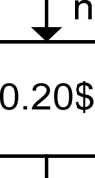
\includegraphics[width=1.26in,height=1.08in]{./image16} &
    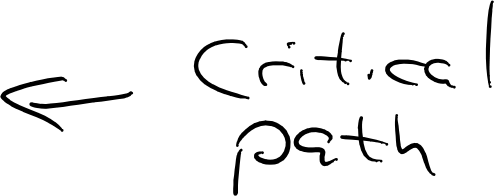
\includegraphics[width=0.747in,height=1.35in]{./image17} &
    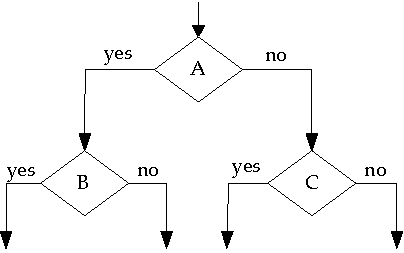
\includegraphics[width=2.16in,height=1.314in]{./image18} \\
    (a) &  (b)  & (c) \\
    \end{tabular}

    \begin{onlysolution}
      \textbf{[R]}
      \itshape
      \begin{verbatim}
        a. while(x) y;
        b. do y while(x);
        c. if (a) {if (b) s1 else s2} else {if (c) s3 else s4}
      \end{verbatim}
    \end{onlysolution}

\item
  Create a flowchart that outlines how to crochet a two-tone blanket
  with a diagonal stripe across it as shown below. A blanket is
  crocheted by linking together a sequence of basic stitches. For the
  purposes of the flowchart assume that a basic stitch is an elaborate
  process. Basic stitches are made from either dark or light yarn. The
  blanket should be 100 stitches wide by 150 stitches high. The diagonal
  stripe runs at a 45 degree angle from the horizontal.

  
\includegraphics[width=1in,height=1.34in]{./image19}

  \begin{onlysolution}
    \textbf{[R]}
    \itshape
    This process starts at the upper left corner of the blanket and proceeds to 
    the right forming one row of 100 basic stitches and then works back to the left 
    forming the second row. This process repeats for the next 148 rows.
    ** Add figures **
  \end{onlysolution}


\item
  Build a data flow diagram and event table to represent an image
  archiving system for an art museum. The art museum maintains a
  database of digital images of paintings from museums all over the
  world. The following information is known about the image database
  system:

\begin{itemize}
\item
  Images are shared among museums in a participating network. Whenever a
  participating museum posts a new image, it sends a broadcast email to
  all participating museums in the network with the image attached as an
  email. It provides the name of the painting and artist in the body of
  the email. All new images received are added directly to the museum's
  own image database.
\item
  When inserted into the museum's database, each image is provided with
  a tag identifying the name of the painting and the artist.
  Furthermore, this triggers an image analysis routine that classifies
  the image based into predefined categories such as portrait, natural
  scene, and modern. Furthermore, it stores key features that are
  extracted from the image.
\item
  The key features are used to identify and retrieve visually similar
  images from the museum's database. Another image processing algorithm
  is run that compares the visual similarity of the new image to all
  images in the database. This process produces a matching score of 0 to
  100 that is stored.
\item
  The museum's image database is available to visitors via computer
  kiosks placed throughout the museum. Kiosk users can retrieve and view
  images in one of three ways. First, they can specify the name of the
  artist or painting. Second, they can retrieve a class of images, such
  as modern. Third, once they have received a painting, they can submit
  a request to view visually similar images. The visually similar images
  are retrieved for viewing based upon the matching score.
\end{itemize}

  \begin{onlysolution}
    \textbf{[R]}
    \itshape
    ** Add figure **
  \end{onlysolution}

\item
  Build an ERD to keep track of the bicycle frames manufactured at a
  local company. The following are notes from an interview with the
  owner.

\begin{quote}
\emph{We custom build bike frames to the dimension of each individual
customer. When a customer comes in we take measurements in their height,
leg length, arm length, torso length, weight, and waist measurement.
Since we have high customer satisfaction our customers order new frames
every several year. Hence we would like to date these measurements in
order to track how a customer's body changes through time .Each frame is
built on one set of measurements. Clearly, we need to keep track of our
customer's contact information like name, address, phone number, and
email address. We would like to know which employee built which frame.
We would like to store basic information like name, address, phone, and
SSN for each employee. Each frame is built by one employee using a
variety of different titanium tubing. We have strict inventory control
on all of our tubing and need to keep track of its grade, lot \#, Outer
Diameter (OD), Inner Diameter (ID), and manufacturer. Tubing is uniquely
identified by its lot \#. Finally we need to keep information on the
frame. Each frame is given a unique serial number, and has a color,
type, and dimensions.}
\end{quote}

\begin{onlysolution}
  \textbf{[R]}
  \itshape

In creating an ERD its typical to “grow” the ERD from a single entity. As a 
starting point, lets consider the frame entity. Clearly, a serial number uniquely 
identifies a particular frame. The type and color of the frame are attributes. 
Its a common mistake for students to list the possible values of the frame type as 
attributes of a frame. This is incorrect, an attribute represents the domain of 
possible values. Is the tubing used to build a frame an attribute or an entity 
itself? Anytime that you can generate a unique identifier for a thing then its a good 
bet that it should be its own entity. In the case of tubing, we can combine the lot#, 
manufacture, and type to distinguish between tubes. We assume that a bike frame is made 
from 1 type of tubing and a particular lot of tubes can be used to build many frames. 
One might be tempted to relate customers and frames, however, there is nothing in the 
word statement that explicitly requires this. Its better to relate frames to the orders 
which generate them. We can then relate customers to their orders. The cardinality of 
these two relationships are clear from the diagram. From the notes gathered its clear 
that we need to store the customer’s name, address, and phone number. These are all 
attributes which help to identify a particular customer. We could use the customers 
name as the primary key, it’s a safe bet that a particular name will not be repeated. 
Finally we need to relate the customer to their measurements. Since the word statement 
states that a customers measurements may change over time, we cannot have a measurement 
attribute, because an attribute is only allowed to take on a single value for a particular 
entity instance. Hence, we need to make a measurement entity and allow each customer to have 
many measurements. Unfortunately, the arm, leg and torso attributes are not sufficient to 
uniquely identify a particular measurement, its possible for different people to have the 
same measurements. In ERD nomenclature, a entity which lacks a good primary key is called a 
weak entity. When converted into a relational database a weak entity "borrows" its primary key 
from the participating entities.
  ** Add figure **
\end{onlysolution}

\item
  Extend Problem~\ref{problem:stateDiagramTapeCartridges}
  to create an ERD that captures data about the tape
  cartridges used in the backup system. Every Sunday night a full backup
  is made of all network drives. A full backup creates an identical copy
  of the network drives on the tape cartridges. Due to the large amount
  of information, a full backup requires many tapes. On the other nights
  of the week an incremental backup is made. An incremental backup
  stores only files modified since the last backup (either full or
  incremental). Incremental backups are much smaller than a full backup,
  and consequently many incremental backups fit on a single tape. A tape
  contains only full or incremental backup information -- the unused
  portion of the last tape used for a full backup is never used to store
  incremental backups. Your company wants to keep track of tapes, full
  backups, and incremental backups. An ID and state should be tracked
  for each tape. For full backups, the system needs to track the
  creation date and the number of tapes used. For an incremental backup
  it should track the date it was made. The relationships between the
  backup type and the tape will capture which tapes participated in
  which backup. (Hint: the state of a tape should be an attribute of the
  tape entity - unformatted, blank, etc. They are not attributes and are
  possible values for the state attribute.)

  \begin{onlysolution}
    \textbf{[R]}
    \itshape
  \end{onlysolution}

\item
  \textbf{Project Application.} Develop behavior models that are
  applicable for describing your system. 
  Table~\ref{table:guidanceModelSelection} is provided to help
  in making the determination as to which models are applicable.

  \begin{onlysolution}
    \textbf{[R]}
    \itshape
    When students define their projects using the functional decomposition 
    method outlined in chapter 5, they typically will use block diagram 
    listing the inputs, outputs and behaviors for the highest levels of 
    abstraction. However, as the lower levels, the use of alternative design 
    models becomes important to formally describe the behavior of their systems. 
    It is not uncommon for students to use several different languages to 
    describe their systems. For example, a group that is building an autonomous 
    robot may use both state diagrams and flow charts to describe their algorithms.
  \end{onlysolution}

\end{enumerate}
